 \section{Parameter optimization}
Before starting the experiments, some average non-extreme values for the parameters had to be chosen. The frame count was set to 100, the mutation rate was set to 1\%, the population size was set to 30, the codon count was set to 20 and the maximum number of wrappings was set to 3. The starting number of generations for a generational algorithm is 50, while the number of generations for a steady-state algorithm is 500. This is because the generational algorithm creates a completely new generation at each turn, while the steady-state algorithm changes only one unit.

The fitness values represent the number of hits during the simulation of a strategy using a dataset which contains 20000 requests. The stopping criteria at every run was reaching the predetermined number of generations.

\subsection{Selection operator}
The first parameter that was optimized was the selection operator. The first selection operator that was considered was the fitness proportional roulette-wheel selection in a generational genetic algorithm, and the second selection operator that was considered was the tournament selection in a steady-state genetic algorithm.

The median fitness in both of these runs was 1907, so the average fitness was used for analysis.

\begin{figure}[H]
	\centering
	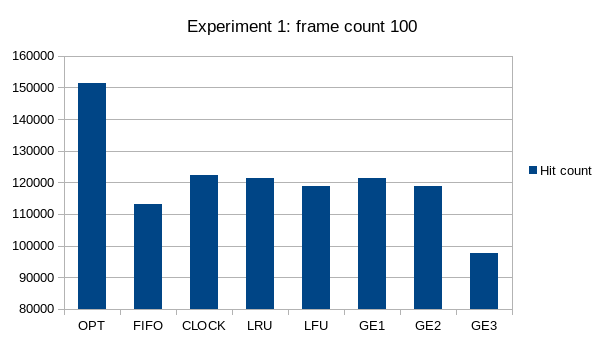
\includegraphics[scale=0.55]{bar_plot_01.png}
	\caption{Results of optimizing the selection operator}
\end{figure}

The roulette-wheel selection had the average fitness of 5325.4, while the tournament selection had the average fitness of 1935.6. The roulette-wheel selection was chosen as the optimal selection operator.

Running 10 experiments using the roulette-wheel selection took about 25 minutes, while running 10 experiments with tournament selection tok about 60 minutes. I believe that both selection operators were given an equal chance, and the roulette-wheel selection cleary emerged as superior.

\subsection{Mutation rate}
The second parameter that was optimized was the mutation rate. Mutation rate was initially set to 1\%, which was shown to be relatively small during the runs comparing the selection operators. So, the tested mutation rates were 1\%, 2\%, 5\%, 10\% and 20\%.

All of these runs had the median fitness of 18999, so the average fitness was used for analysis.

\begin{figure}[H]
	\centering
	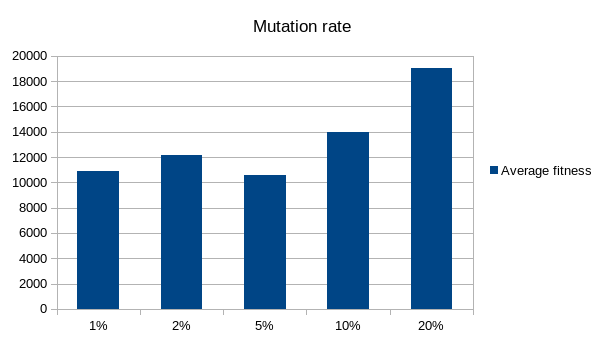
\includegraphics[scale=0.55]{bar_plot_02.png}
	\caption{Results of optimizing the mutation rate}
\end{figure}

The mutation rate of 20\% was chosen as optimal the mutation rate.

\subsection{Population size}
The third parameter that was optimized was the population size. The values that were compared during these runs were the sizes of 10, 30 and 50.

\begin{figure}[H]
	\centering
	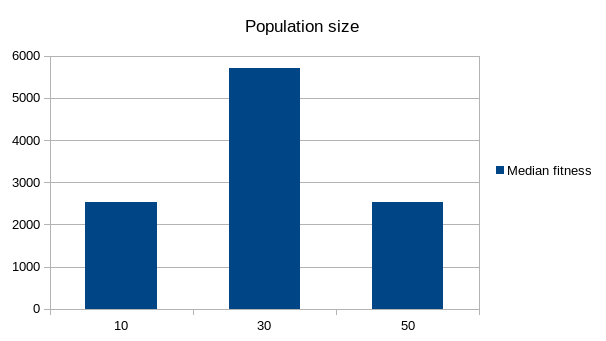
\includegraphics[scale=0.55]{bar_plot_03.png}
	\caption{Results of optimizing the population size}
\end{figure}

The population size of 30 was chosen as the optimal population size.

\subsection{Codon count}
The fourth parameter that was optimized was the codon count. The values that were compared during these runs were the codon counts of 10, 20 and 30.

\begin{figure}[H]
	\centering
	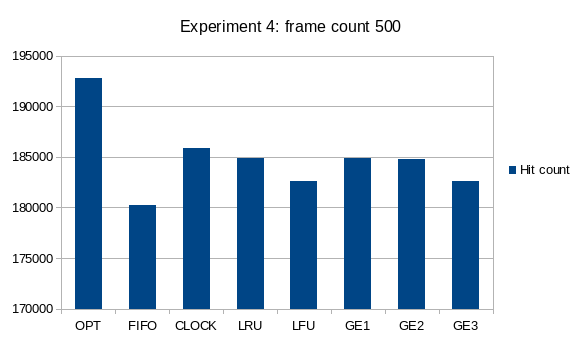
\includegraphics[scale=0.55]{bar_plot_04.png}
	\caption{Results of optimizing the population size}
\end{figure}

Both the runs with the codon count set to 20 and 30 has the median fitness of 5713. The run where the codon count was set to 20 had the average fitness of 9642.3, and the run where the codon coun was set to 30 had the average fitness of 9243.7. Since the first run had higher average fitness, the value 20 was chosen as the optimal codon count. I suspect that the codon count has little significance to the result.

\subsection{Maximum number of wrappings}
The fifth and final parameter that was optimized was the maximum number of wrappings. The values that were compared during these runs were 0, 3 and 5.

\begin{figure}[H]
	\centering
	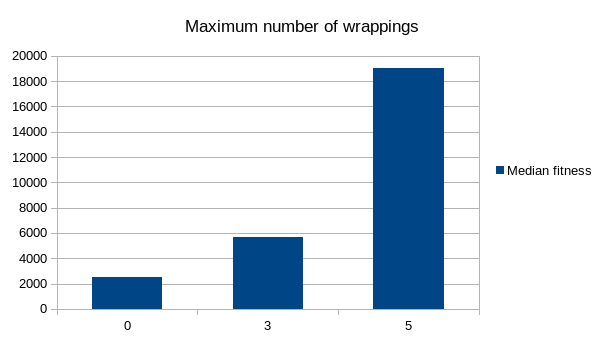
\includegraphics[scale=0.55]{bar_plot_05.png}
	\caption{Results of optimizing the maximum number of wrappings}
\end{figure}

The value 5 was chosen as the optimal value for the maximum number of wrappings.